\documentclass[a4paper]{article}

\usepackage{cite}%多个文献引用
\usepackage{graphicx}
\usepackage{array}%调节表格行高
\usepackage{multirow,makecell}%多行表格
\usepackage{tabularx}%表格固定列宽
\usepackage{subfigure}
\usepackage{titlesec}%标题格式设置
\usepackage{amsmath}
\usepackage{mathtools}
\usepackage{amssymb}
\usepackage{tabularx}
\usepackage{makecell}
\usepackage{geometry}
\usepackage{float}
\usepackage{setspace}%行距包
\usepackage{siunitx}
\usepackage{mdwlist}
\usepackage{tabu}
\usepackage{indentfirst}
\usepackage{enumerate}
\usepackage{setspace} 
\usepackage[super,square]{natbib}

\bibliographystyle{unsrt}
\setlength{\parindent}{2em}

\geometry{top=1.54cm,bottom=2.54cm,left=2.5cm,right=2.5cm}

\begin{document}
\begin{center}
\bf\Large
EE 105 Feedback Control Systems\par
Department of Electrical and Computer Engineering\par
Tufts University Fall 2018\par
Final Project\par   
\end{center}
\begin{table}[H]
\begin{center}
\begin{tabular*}{\textwidth}{@{\extracolsep{\fill}}lcr}
Name: {\it Shang Wang} &Student ID: {\it 1277417} &E-mail: {\it shang.wang@tufts.edu}\\
\hline
\end{tabular*}
\end{center}
\end{table}

% \begin{figure}[H]
% \centering
% 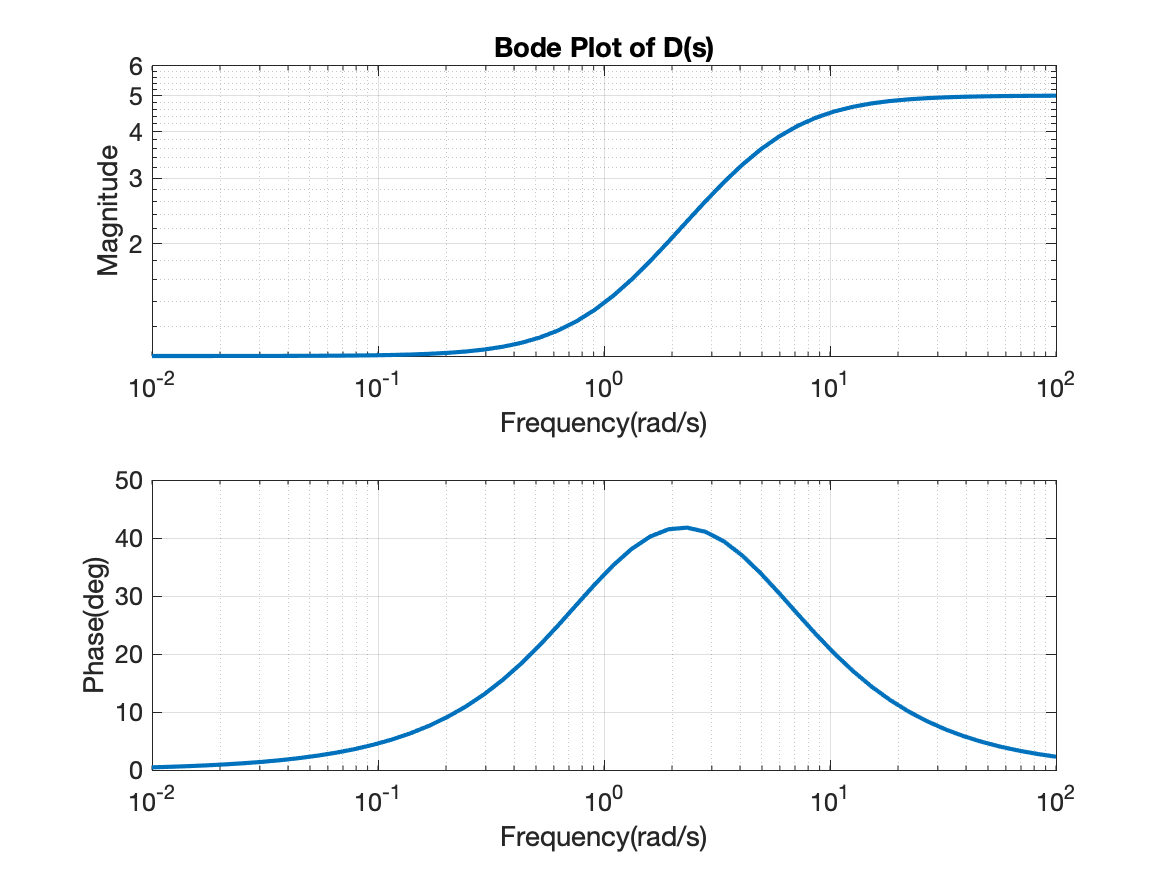
\includegraphics[width = 0.75\textwidth]{pic/0.png}
% \end{figure}

% $$
% A = 
% \left [
% \begin{matrix}
%    -1 & 0 \\
%    1 & 0
% \end{matrix}
% \right ],\ \ \
% $$

% \begin{equation*}
% f_U(u) = 
% \left\{
% \begin{aligned}
% & 0 &&,\ uL-5\\
% & \frac{u+5}{8} &&,\ -5\leq u < -3\\
% \end{aligned}
% \right.
% \end{equation*}

\begin{center}
\Large\bf PD Controller for A Two-Joint Robotic Arm
\end{center}
\setlength{\baselineskip}{1.3\baselineskip}


\begin{abstract}
Robotics is an interdisciplinary with broad prospects and rapid development. The design of its control system is at the heart of robotics. But at the same time, the robot system as a nonlinear, uncertain system has many difficulties in modeling. To solve such problems, many different control methods have been gradually invented. In this paper, a simple two-joint robot arm is modeled, a PD controller is designed and simulated, and finally the Lyapunov stability criterion is used to judge the stability of the system.
\end{abstract}
\begin{center}
\small{{\bf Keywords: }Robotics, Nonlinear control, Lyapunov criterion}
\end{center}



\section{Introduction}

The discipline of robotics is a rapidly developing comprehensive frontier discipline that is highly valued by industry and academia. The foundation of a robot is its control system. From the perspective of control engineering, a robot is a highly nonlinear and not determined system, which adds a lot of difficulty to engineers endeavoring to learn to study robots. In recent years, research in the field of robot control has focused on intelligent control, the direct application of classic control is limited. But the understanding of classical control theory is crucial for high-level control designer. \par

The dynamics of a typical robot arm system could be described by a second order nonlinear differential equation:  
\begin{equation}
\boldsymbol{M(q)\ \ddot{q}}+\boldsymbol{C(q,\dot{q})\ \dot{q}}+\boldsymbol{G(q)} + \boldsymbol{F(\dot{q} )} + \boldsymbol{\tau_d} = \boldsymbol{\tau}
\label{robot dynamics}
\end{equation}
In which, $\boldsymbol{q}\in \mathbb{R}^{n}$ is the displacement of each joint, $\boldsymbol{M(q)}\in \mathbb{R}^{n\times n}$ is a matrix related to the mass and moment of inertia of the robot arm, $\boldsymbol{C(q,\dot{q})}\in \mathbb{R}^{n\times n}$ refers to centrifugal force and Coriolis force of the robot, $\boldsymbol{G(q)}\in \mathbb{R}^{n}$ is gravitational term, $\boldsymbol{F(\dot{q})}\in \mathbb{R}^n$ is friction, $\boldsymbol{\tau_d} \in \mathbb{R}^n$ is disturbance that is likely to have any form, last one $\boldsymbol{\tau} \in \mathbb{R}^n$ is driving torque of each joint\cite{ref1}.

A typicl two joint arm, which is also the research entity of this essay, is like: 
\begin{figure}[H]
\centering
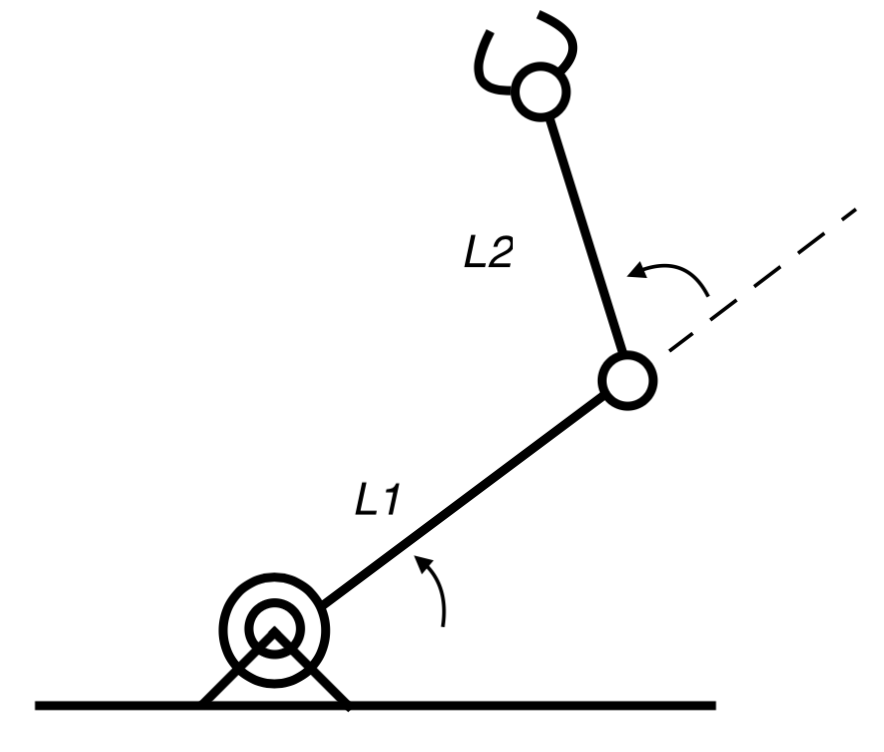
\includegraphics[width = 0.2\textwidth]{pic/robo.png}
\caption{Robotic Arm}
\end{figure}

In this essay, a model of this robot will be derived and transfered into form like Eq(\ref{robot dynamics}). The stability of the system will be analyzed by using the Lyapunov stability criterion. Then, a simulink simulation model will be built to evaluate its transient performance.

\subsection{Introduction of Lyapunov Stability Criterion}

Lyapunov stability criterion is one of few methods that can directly applied to nonlinear system. A notable feature of this method is that the stability of the system can be judged without solving the differential equation of the control system. However, it should be noted that this method can judge the stability of the system, but it does not provide any information about the transient response or system performance. More concretely, this method can neither give information that the system is overdamped or underdamped, nor can it give the time when the system reaches its steady state. That is, even if the system is stable, the performance of the system may be unsatisfactory. 

Lyapunov stability criterion is used to decide the stability of the following differential equation\cite{ref2}:
\begin{equation}
\boldsymbol{\dot{X}} = f(\boldsymbol{X})
\label{differential equation}   
\end{equation}

In which $\boldsymbol{X}\in \mathbb{R}^n$, function $f(\boldsymbol{X})$ could be a nonlinear function in any form. Similarly to the methed when we use to find state variables in control system, a high order diffrential equation can always be organaized as a set of first order differential equation like Eq(\ref{differential equation}). The first step to judge the stability of a nonlinear system is to struct a generalized energy function $v(\boldsymbol{X})$ with following feathers
\begin{enumerate}
   \item $v(\boldsymbol{X})$  has a continuous first-order partial derivative. For any $\boldsymbol{X}\neq \boldsymbol{0}$, $v(\boldsymbol{X}) > 0 $.
   \item $\dot{v}(\boldsymbol{X})\leq 0$, in which $\dot{v}(\boldsymbol{X})$ is the derivative in any possible trajectory of the system.
\end{enumerate}
 
One thing has to be noticed is that the system is a weakly stable system if features above can only be satisfied in particular region. Relatively, the stability of the system is strong only if these features are established on all domains. In the perspective of physics, if the system has a positive energy function and its value is always attenuated or kept constant, then the system is stable, in other words, the state variables of the system have certain boundaries. 

Especially, the state variables will converge progressively to $\boldsymbol{0}$ when $\dot{v}(\boldsymbol{X})< 0$. Correspondingly, when $\dot{v}(\boldsymbol{X})\leq 0$, 
the system might be stabilized at some point where $v(\boldsymbol{X})\neq 0$. The particular value of that point need to be determined in such case. 


\subsection{Introduction of System Function}

S-function(system function) module is the core of the entire simulink dynamic system. Users can write S-Functions by using  languages such as matlab script, C, C++, Fortran, etc. S-Function consists of a specific syntax that describes and implements dynamic systems such as continuous systems, discrete systems, or composite systems. It offers users a platform to customize their own dynamic systems and provides an interface between the hardware and simulink solver.  A complete structure of S-Function contains all the capabilities needed to describe a dynamic system. All other use cases are specific usage of this structure. 

A complete S-function structure includes several functional modules such as initialization(\emph{mdlInitializeSizes}), derivative of the state variables(\emph{mdlDerivatives}), outputs of the system(\emph{mdlOutputs}) etc. Please refer to the matlab manual for specific uses of S-Function. 


\subsection{Commonly used Control Methedology}
The main purpose of the robot control system is to make sure the position and velocity of each joint is tracking a set of given coordinates as much as possible by means of applying torque to each joint. \par

There are some commonly used methods. 
\begin{enumerate}
   \item The methodology based on the precise dynamics model of the system. Classic methods, such as compensator design, can be implemented in some case that the system is able to be linearized. The drawback is obvious that the precise model of a real robot is almost impossible to derive. 
   \item PID control is widely used in robot control with advantages that the control law is simple, easy to implement, and does not require modeling. But at the same time, the transient performance and control energy cost are not guaranteed. 
   \item Adaptive controller can correct its own parameters in time to adapt to the dynamics of the controlled object and external disturbances, so that the entire control system always has satisfactory performance. But the weakness is that it requires a lot of computation and has high requirements for real-time performance. Apart from that, the control law is often complicated.
   \item Robust control is such a method that can ensure the stability of undetermined system so as to achieve adequate performance. The only thing that a robust controller designer needs to know is the boundary of the uncertainty of the parameters. It’s easy for the designer compared to the adaptive controller since the control law is always simple. 
   \item Neural network control and fuzzy control have the ability to approximate nonlinearity. The development of this technology opens up a new way to design a controller for complex nonlinear and uncertain systems.
   \item Iterative learning control is a branch of intelligent control with rigorous mathematical description, which is suitable for solving high-precision control problems with strong nonlinearity, strong coupling and having difficulty in modeling. Iterative learning controller has simpler form and requires less prior knowledge. 
\end{enumerate}



\section{Modeling and Calculations}

Consider the two joint robot mentioned before, its dynamics can be expressed by a set of differential equations. This is a typical and simplest robotic arm. Studying this model has important inspiration and guidance for designing other more complex robot structures and robot controller. Before calculation, we need to simplify the model first.
\begin{enumerate}
   \item There is no friction of any kind.
   \item The mass is concentrated at the end of each arm(link).
\end{enumerate}

% \begin{figure}[H]
% \centering
% 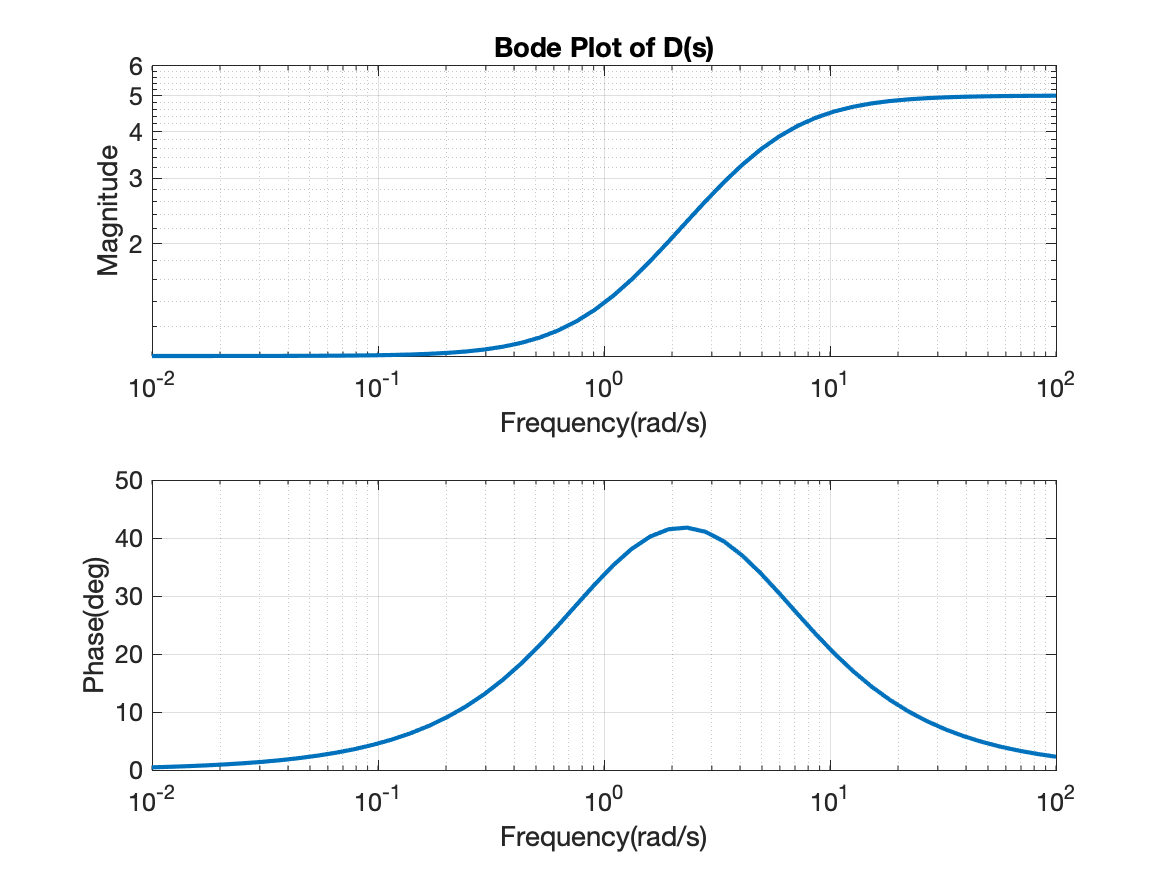
\includegraphics[width = 0.75\textwidth]{pic/0.png}
% \end{figure}

There are two methods to derive a full description of the dynamics of a robot system. 

\begin{enumerate}
   \item Newton's Euler iterative dynamic equation: The fondation of this theory are Newton's second law and the famous Newton-Euler equation. It's a classic algorithm based on balancing force. 
   \item Lagrangian Function: is another famous eqaution based on the energy of the system, which provides a methods to derive the dynamics of the system by a Scalar Valued Function. 
\end{enumerate}

In this essay, the dynamics of the system is established by using the Lagrangian function. 
\begin{equation}
   \boldsymbol{\mathcal{L}(\boldsymbol{\Theta},\boldsymbol{\dot\Theta})} = \boldsymbol{k(\Theta,\dot\Theta)}-\boldsymbol{u(\Theta)}
\end{equation}

In which, $\boldsymbol{k(\Theta,\dot\Theta)}$ refers to the kenetic energy and $\boldsymbol{u(\Theta)}$ is the potential energy. It turns out for each link of the robot, the dynamic function\cite{ref3}
\begin{equation}
   \frac{\rm d}{{\rm d}t}\frac{\partial\mathcal{L}_i}{\partial\dot\Theta_i} - \frac{\partial\mathcal{L}_i}{\partial\Theta_i} = \tau_i
\end{equation}
Where $\tau_i$ is the torque need to be applied to the $i$-th joint. More specifically,
\begin{equation}
   \frac{\rm d}{{\rm d}t}\frac{\partial k_i}{\partial\dot\Theta_i} - \frac{\partial k_i}{\partial\Theta_i} + \frac{\partial u_i}{\partial \Theta_i} = \tau_i
   \label{Lagrangian}
\end{equation}

Create a coordinate system as shown below:
\begin{figure}[H]
\centering
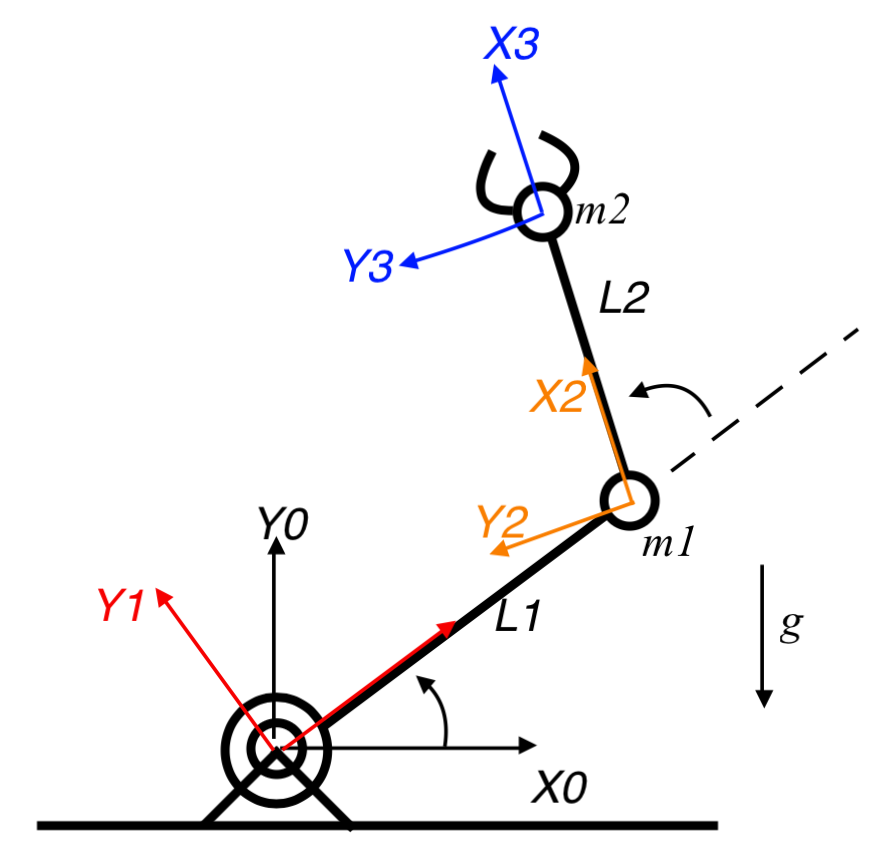
\includegraphics[width = 0.2\textwidth]{pic/cor.png}
\caption{Coordinates}
\end{figure}
\par
The kenetic energy of the $i$-th link is 
\begin{equation}
k_i = \frac{1}{2} m_i \boldsymbol{v}_{C_i}^T \boldsymbol{v}_{C_i}^{} + \frac12 \prescript{i}{} {\boldsymbol{\omega}}_i^T \prescript{C_i}{}{\boldsymbol{I}_i} \prescript{i}{}{\boldsymbol{\omega}}_i
\label{kenetics}
\end{equation}
Where the first term is the kenetic energy related to the velocity of the mass center of the $i$-th link, the second term is the kinetic energy contributed by the angular velocity of the link relative to the axis passing through the center of mass. So in this model, the kenetic energy of the first link is 
$$
k_1 = \frac 12 m_1l_1^2\dot{\theta}_1^2
$$

However, the solution of the second link is not as simple as this. This problem can be solved by geometric methods. But in this place we use a more extensive approach. First, find the rotation matrics between each coordinate system
\begin{equation}
  \prescript{0}{1}{\boldsymbol {R}}   = 
\left [
\begin{matrix}
   c_1 & -s_1 & 0  \\
   s_1 & c_1 & 0 \\
   0 & 0 & 1 \\
\end{matrix}
\right ],\ \ \
\prescript{1}{2}{\boldsymbol {R}}   = 
\left [
\begin{matrix}
   c_2 & -s_2 & 0 \\
   s_2 & c_2 & 0 \\
   0 & 0 & 1  \\
\end{matrix}
\right ],\ \ \
\prescript{2}{3}{\boldsymbol {R}}  = 
\left [
\begin{matrix}
   1 & 0 & 0  \\
   0 & 1 & 0  \\
   0 & 0 & 1  \\
\end{matrix}
\right ]
\end{equation}
(note: for the sake of simplicity, $c_1$ refers to $\cos\theta_1$ and $s_{12}$ refers to $\sin(\theta_1+\theta_2)$, other similar notaions refer to the conresponding trigonometric functions as well)
Then we can get the velocity $\prescript{1}{}{\boldsymbol{v}}_1$ and the angular velocity $\prescript{1}{}{\boldsymbol{\omega}}_1$ of the origin of coordinate system \{1\} described in itself. 
\begin{equation}
\prescript{1}{}{\boldsymbol{v}}_1 = 
\left [
\begin{matrix}
   0  \\
   0 \\
   0  \\
\end{matrix}
\right ],\ \ \
\prescript{1}{}{\boldsymbol{\omega}}_1 = 
\left [
\begin{matrix}
   0  \\
   0 \\
   \dot\theta_1 \\
\end{matrix}
\right ]
\end{equation}

\noindent Next, the velocity $\prescript{2}{}{\boldsymbol{v}}_2$ and the angular velocity $\prescript{2}{}{\boldsymbol{\omega}}_2$.

\begin{equation}
\prescript{2}{}{\boldsymbol{v}}_2 = 
\left [
\begin{matrix}
   c_2 & -s_2 & 0  \\
   s_2 & c_2 & 0 \\
   0 & 0 & 1 & \\
\end{matrix}
\right ]^{-1}
\left [
\begin{matrix}
   0  \\
   l_1\dot{\theta}_1\\
   0  \\
\end{matrix}
\right ] = 
\left [
\begin{matrix}
   l_1s_2\dot\theta_1  \\
   l_1c_2\dot\theta_1\\
   0  \\
\end{matrix}
\right ],\ \ \
\prescript{2}{}{\boldsymbol{\omega}}_2 = 
\left [
\begin{matrix}
   0  \\
   0 \\
   \dot\theta_1+ \dot\theta_2 \\
\end{matrix}
\right ]
\end{equation}
\noindent Go through the similar process
\begin{equation}
\prescript{3}{}{\boldsymbol{v}}_3 = 
\left [
\begin{matrix}
   l_1s_2\dot\theta_1  \\
   l_1c_2\dot\theta_1 + l_2(\dot\theta_1 + \dot\theta_2)  \\
   0  \\
\end{matrix}
\right ],\ \ \
\prescript{3}{}{\boldsymbol{\omega}}_3 = 
\left [
\begin{matrix}
   0  \\
   0 \\
   \dot\theta_1+ \dot\theta_2 \\
\end{matrix}
\right ]
\end{equation}

\noindent We can get the velocity $\prescript{0}{}{\boldsymbol{v}}_3$:
\begin{equation}
\prescript{0}{}{\boldsymbol{v}}_3 = \prescript{0}{3}{\boldsymbol{R}}\prescript{3}{}{\boldsymbol{v}}_3 =
\left [
\begin{matrix}
   -l_1s_1\dot\theta_1-l_2s_{12}(\dot\theta_1+\dot\theta_2)  \\
   l_1c_1\dot\theta_1+l_2c_{12}(\dot\theta_1+\dot\theta_2) \\ 
   0 \\
\end{matrix}
\right ]   
\end{equation}

In the field of robotics, this process above is called forward kenetics , which is a directly application of mechenics and linear algebra. This method aims at solving all the velocity related to each joint with respect of the world coordinates \{0\}. 

Thus, according to Eq(\ref{kenetics})
\begin{equation}
   k_2 = \frac{1}{2} m_2 \prescript{0}{}{\boldsymbol{v}}_{3}^T \prescript{0}{}{\boldsymbol{v}}_3
\end{equation}
Since the mass only exists at the end of the second link $L_2$, which directly leads to that the Inertia Matrics $\boldsymbol{I}$ is zero matrics, in other words, the second term in Eq(\ref{kenetics}) is zero. 

The potential energy 
\begin{equation}
\boldsymbol{u}(\Theta) = 
\left[
\begin{matrix}
m_2l_2gc_{12}+(m_1+m_2)l_1gc_1  \\
m_2l_2gc_{12} \\
\end{matrix}
\right ]
\end{equation}

So far, the dynamic function of this robot system could be built in the form represented in Eq(\ref{robot dynamics}) by Lagrangian function Eq(\ref{Lagrangian}). 
\begin{equation}
\boldsymbol{M(\Theta) \ddot{\Theta}}+\boldsymbol{C(\Theta,\dot{\Theta})\dot{\Theta}}+\boldsymbol{G(\Theta)} = \boldsymbol{\tau}  
\label{robot arm}
\end{equation}
Where
\begin{equation}
\boldsymbol{M(\Theta)} = 
\left[
\begin{matrix}
l_2^2+2l_1l_2m_2c_2+l_1^2(m_1+m_2) &l_2^2m_2+l_1l_2m_2c_2  \\
l_2^2m_2+l_1l_2m_2c_2 &l_2^2m_2 \\
\end{matrix}
\right ]
\end{equation}
\begin{equation}
\boldsymbol{C(\Theta,\dot{\Theta})} = 
\left[
\begin{matrix}
-m_2l_1l_2s_2\dot\theta_2 & -m_2l_1l_2s_2(\dot\theta_1+\dot\theta_2)  \\
m_2l_1l_2s_2\dot\theta_1 & 0 \\
\end{matrix}
\right ]
\end{equation}
\begin{equation}
\boldsymbol{G(\Theta)} = 
\left[
\begin{matrix}
m_2l_2gc_{12}+(m_1+m_2)l_1gc_1  \\
m_2l_2gc_{12} \\
\end{matrix}
\right ]
\end{equation}

It can be seen that one of the simplest robot models requires a nonlinear and complex equation to discribe its dynamics, which compels the computational cost of the classical control compensator design becomes unaffordable. In order to evaluate the stability and performance of such a system, nonlinear control theory needs to be applied. 



\section{Control System Design and Simulations}

Considering a linear system, many methods such as Root Locus, Nyquist, state space method, etc. can be used to analyze system performance and design compensators. For systems with inconspicuous nonlinear features, such as single pendulum systems, local linearization can be used to approximate nonlinear equations near the operating point. Unfortunately, for systems such as robotic arms that operate over a wide range of workspaces, the method of local linearization does not apply. Therefore, for this case, the controller can be designed directly using a nonlinear method. 

\subsection{Control System Design}

The control law of a joint independent PD controller is as follows
\begin{equation}
\boldsymbol{\tau} = \boldsymbol{K}_p\boldsymbol{e} + \boldsymbol{K}_d\boldsymbol{\dot e}
\end{equation}
Where $\boldsymbol {e} = \boldsymbol{\Theta}_d - \boldsymbol{\Theta}$, $\boldsymbol{K}_d$ and $\boldsymbol{K}_d$ are positive diagonal matrics. It is worth noting that this controller does not allow the robotic arm to track a particular trajectory, but can reach the target position along a trajectory determined by the dynamics of the system. 
If we assume that we have aleady the garavity-related term $\boldsymbol{G(\Theta)}$, a controller including gravity compensation should be
\begin{equation}
\boldsymbol{\tau}_g = \boldsymbol{K}_p\boldsymbol{e} + \boldsymbol{K}_p\boldsymbol{\dot e} + \boldsymbol{G(\Theta)}
\label{gravity}
\end{equation}
The dynamics of the close loop system is(combined Eq(\ref{robot arm}) and Eq(\ref{gravity}))
\begin{equation}
-\boldsymbol{K}_d \boldsymbol{\dot e}= \boldsymbol{M(\Theta) \ddot{\Theta}}+\boldsymbol{C(\Theta,\dot{\Theta})\dot{\Theta}} + \boldsymbol{K}_p\boldsymbol{e}
\label{control}
\end{equation}
For position control only, $\boldsymbol{\Theta}_d$ is constant, therefore $\boldsymbol{\dot\Theta}_d = \boldsymbol{\ddot\Theta}_d \equiv 0$. So Eq(\ref{control}) becomes:
\begin{equation}
-\boldsymbol{K}_d \boldsymbol{\dot e}= \boldsymbol{M(\Theta) \ddot{e}}+\boldsymbol{C(\Theta,\dot{\Theta})\dot{e}} + \boldsymbol{K}_p\boldsymbol{e}
\end{equation}
From which we can generate a Lyapunov function
\begin{equation}
\boldsymbol{V} = \frac 12 \boldsymbol{\dot e}^T\boldsymbol{M}\boldsymbol{\dot e} + \frac 12 \boldsymbol{e}^T\boldsymbol{K}_p\boldsymbol{e} 
\end{equation}
Obviously, $\boldsymbol{V}$ is positive-definite Matrics since $\boldsymbol{K}_p$ and $\boldsymbol{M}$ are positive. Then
\begin{equation}
\boldsymbol{\dot V} = \boldsymbol{\dot e}^T\boldsymbol{M}\boldsymbol{\ddot e} + \frac 12 \boldsymbol{\dot e}^T\boldsymbol{\dot M}\boldsymbol{\dot e} + \boldsymbol{\dot e}^T\boldsymbol{K}_p\boldsymbol{e} 
\end{equation}
There is a useful equation here, which can be derived from the langrangian function of the robot system{\cite{ref2}}.
\begin{equation}
\boldsymbol{\dot e}^T\boldsymbol{\dot M}\boldsymbol{\dot e}  = 2\boldsymbol{\dot e}^T\boldsymbol{C}\boldsymbol{\dot e} 
\end{equation} 
Then
\begin{equation}
\boldsymbol{\dot V}  = \boldsymbol{\dot e}^T(\boldsymbol{M}\boldsymbol{\ddot e} + \boldsymbol{C}\boldsymbol{\dot e} + \boldsymbol{K}_p\boldsymbol{e}) = -\boldsymbol{\dot e}^T\boldsymbol{K}_d\boldsymbol{\dot e} \leq 0
\end{equation}
Now we need to discuss whether the state variable of the closed-loop system Eq(\ref{control}) can converge to zero when the $\boldsymbol{\dot V}$ is zero. In this case, the necessary conditions for a stable system are $\boldsymbol{\dot \Theta} = \boldsymbol{\ddot \Theta}  = 0$. According to Eq(\ref{control})
\begin{equation}
\boldsymbol{K}_p \boldsymbol{e} = \boldsymbol{0} 
\end{equation}
$\boldsymbol{e} = \boldsymbol{0}$ for $\boldsymbol{K}_p$ is not zero matrics. So this system is progressively stable in all domain. 

\subsection{Simulation}
Now we can apply this control law Eq(\ref{gravity}) to the robot arm system Eq(\ref{robot arm})and run a simulation. 
\begin{figure}[H]
\centering
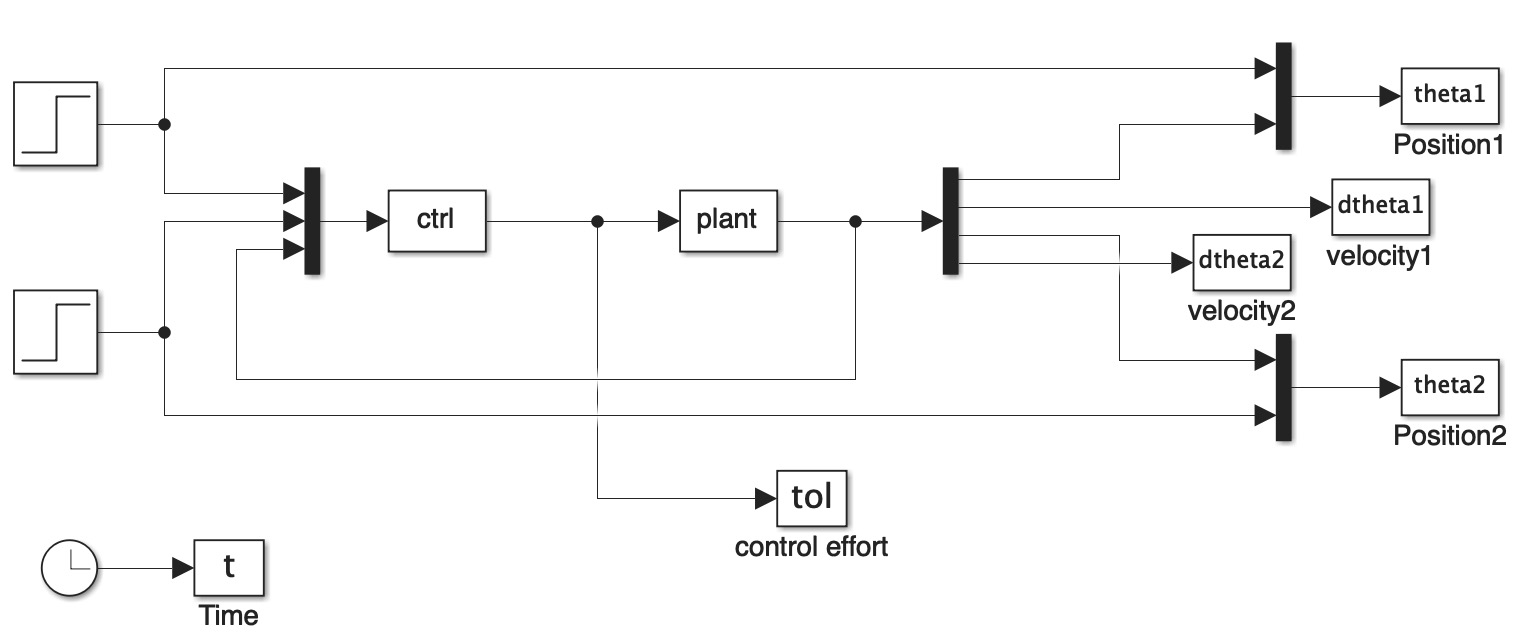
\includegraphics[width = 0.5\textwidth]{pic/sim.png}
\caption{Simulation Block Diagram}
\end{figure}
And the step resopnse 

\begin{figure}[H]
\centering
\begin{minipage}[t]{0.48\textwidth}
\centering
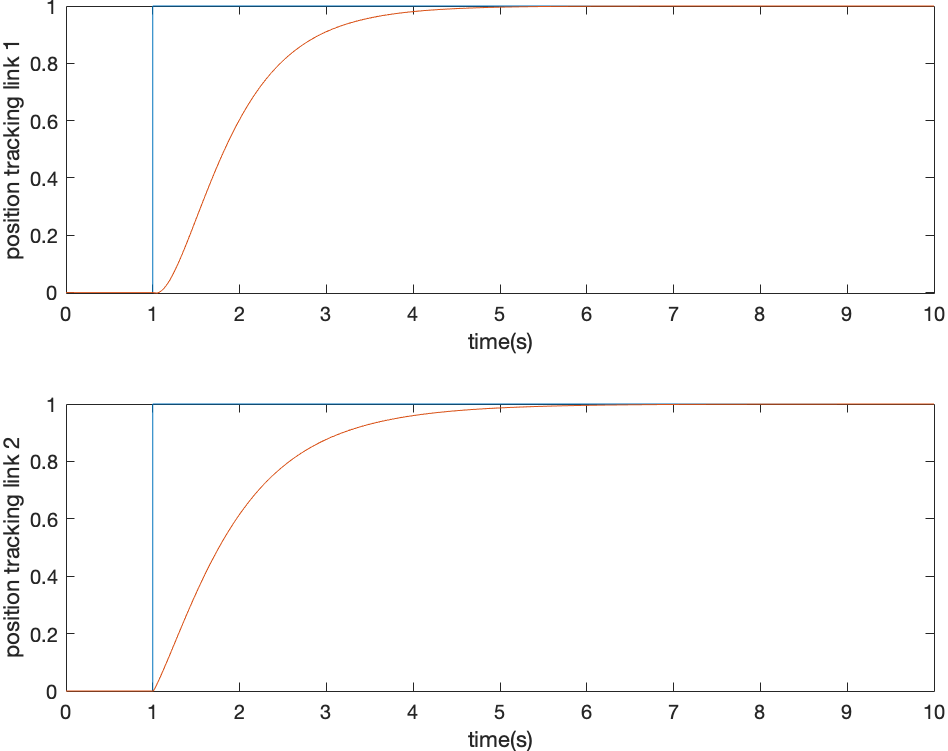
\includegraphics[width=\textwidth]{pic/pos.png}
\caption{Position response}
\end{minipage}
\begin{minipage}[t]{0.48\textwidth}
\centering
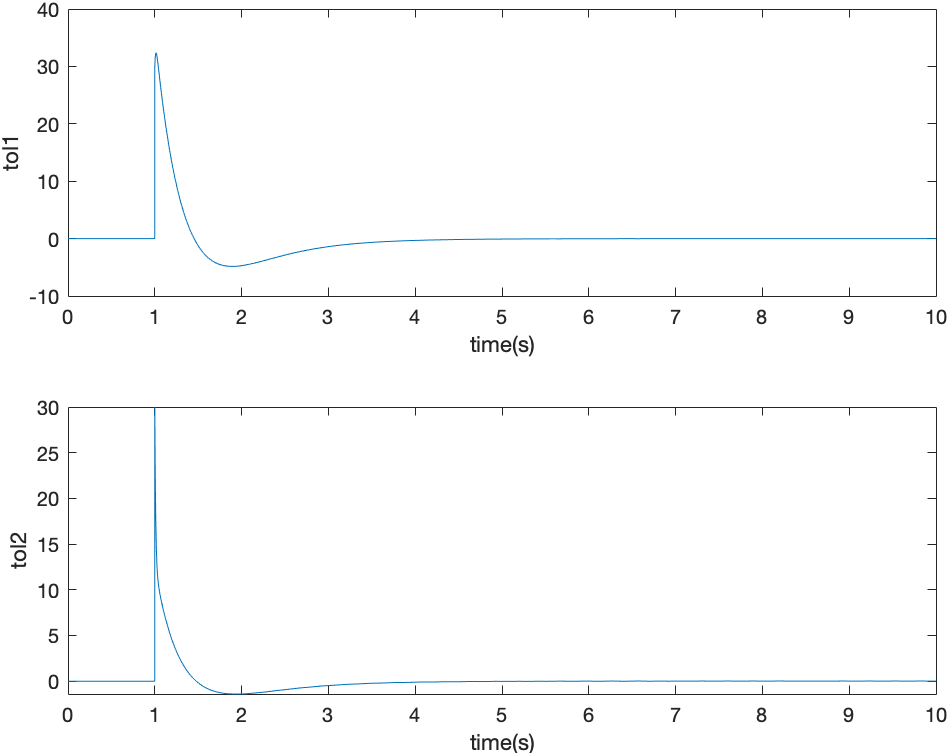
\includegraphics[width=\textwidth]{pic/tol.png}
\caption{Control effort}
\end{minipage}
\end{figure}

% \begin{figure}[H]
% \centering
% 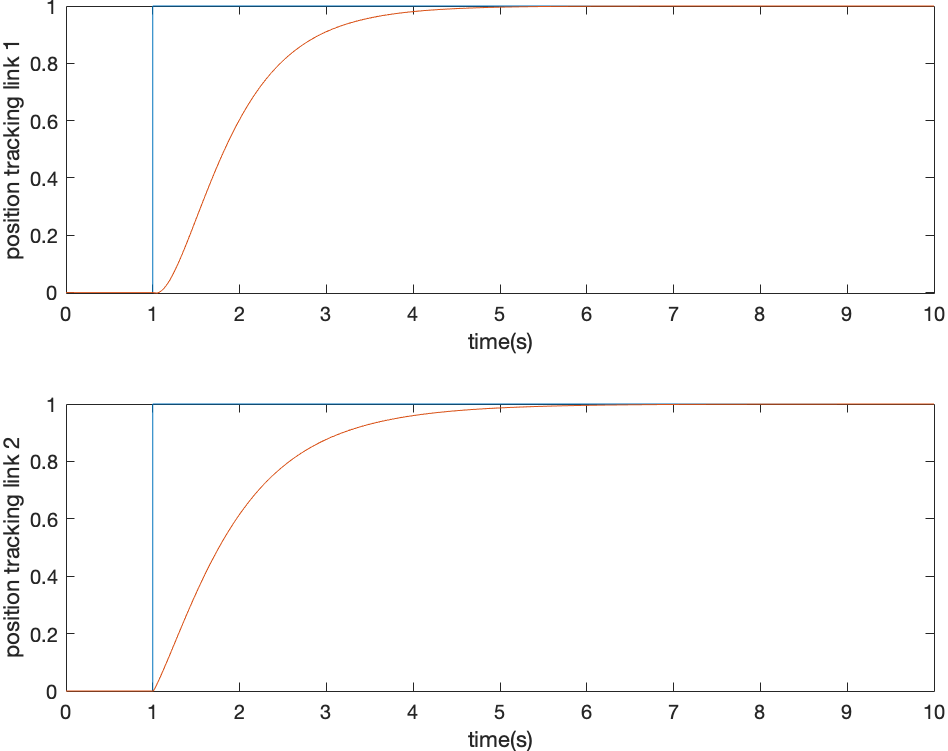
\includegraphics[width = 0.5\textwidth]{pic/pos.png}
% \end{figure}

% % \begin{figure}[H]
% % \centering
% % 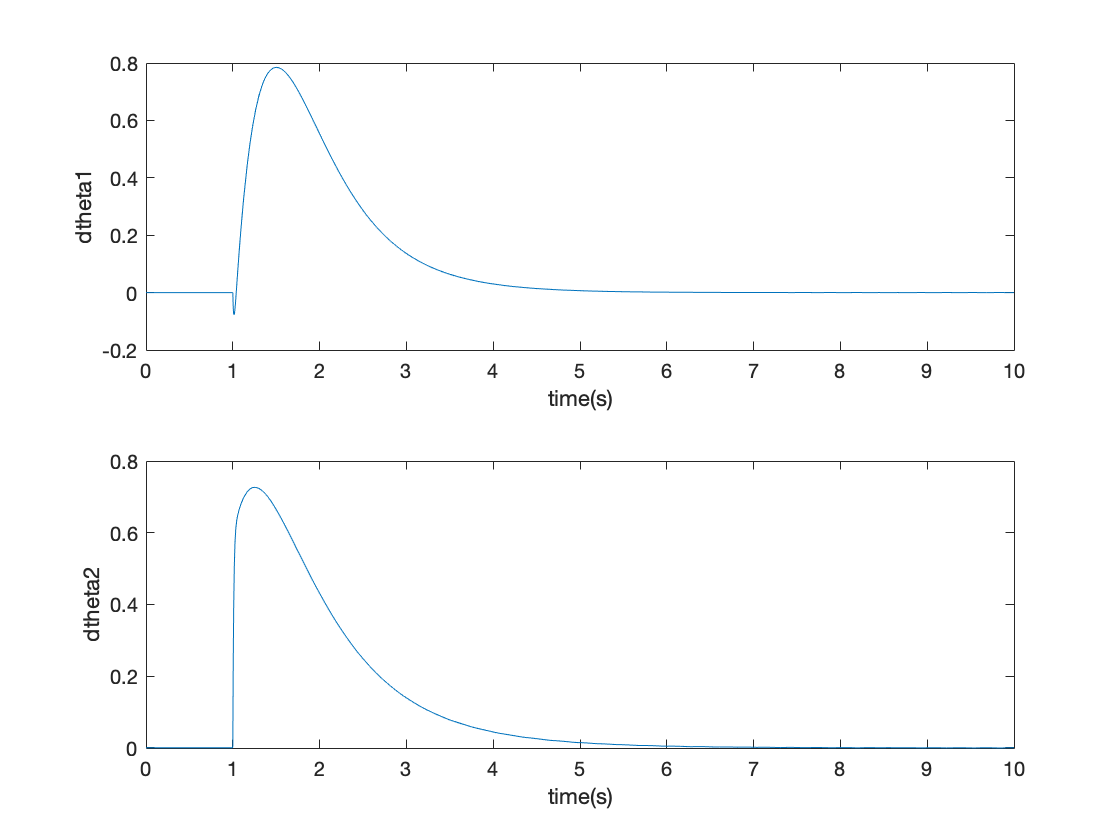
\includegraphics[width = 0.5\textwidth]{pic/v.png}
% % \end{figure}

% \begin{figure}[H]
% \centering
% 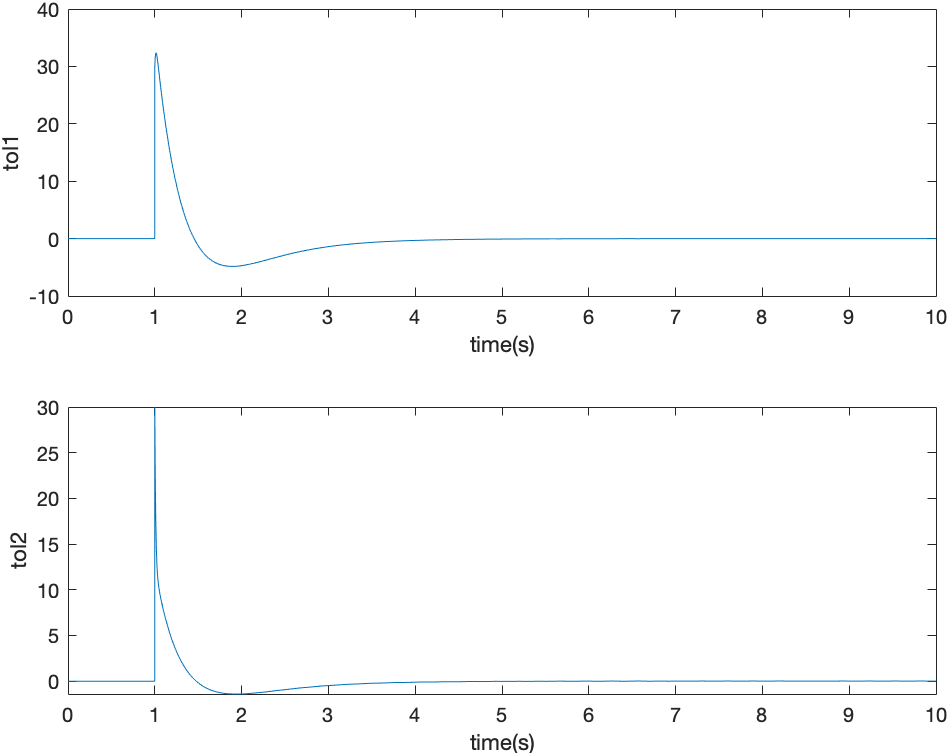
\includegraphics[width = 0.5\textwidth]{pic/tol.png}
% \end{figure}

We can see that the simulation results of the robot arm are satisfactory under conditions $\boldsymbol{K}_p>0$ and $\boldsymbol{K}_d>0$. Properties like rising time, overshoot, etc, can be manipulated by changing its gain. As we expected before, this controller has poor ability of tracking trajactories. 

\begin{figure}[H]
\centering
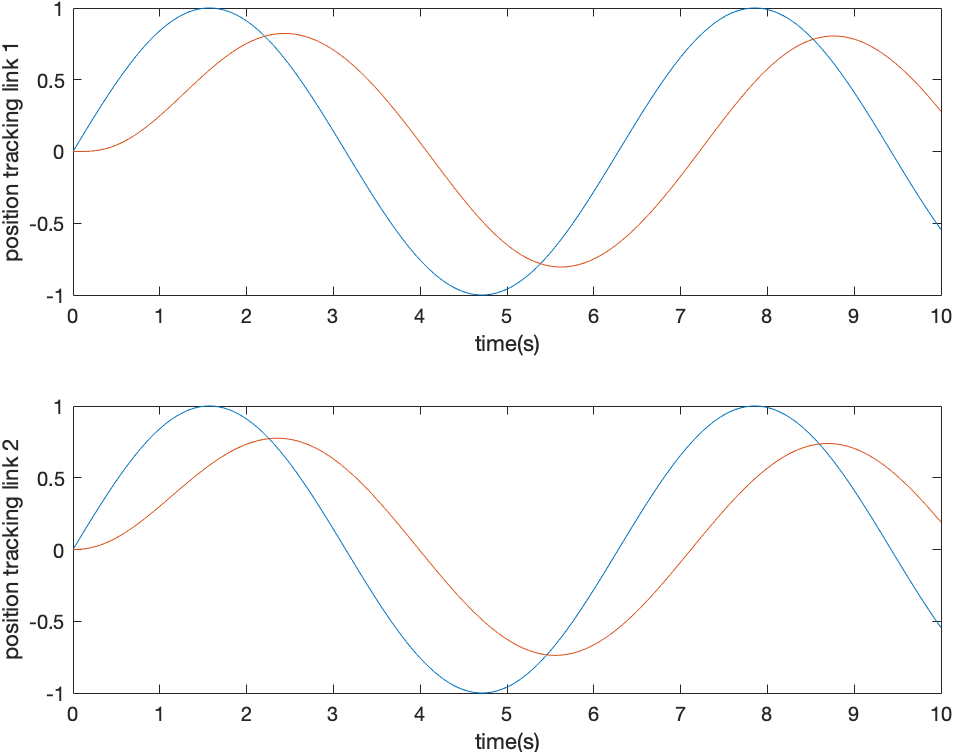
\includegraphics[width = 0.5\textwidth]{pic/sin.png}
\caption{Position respend to sinusoidal inputs}
\end{figure}

It must be clarified that the above process relies on accurate modeling of the robot arm, but the modeling process does not take into account factors including but not limited to modeling errors, friction and external disturbances. In practical applications, when considering various practical factors, it turns out that the exact form of many disturbance terms remain unknown. At this time, it is necessary to adopt the above-mentioned more advanced control methods, such as letting the controller continuously learn to adapt to the control of the disturbance item. 

\section{Conclusion}
In this paper, a simple two-degree-of-freedom robot arm is modeled, its dynamic equation is derived, and a simple PD controller is constructed to realize the function of position control. Moreover, the stability of the closed-loop system is judged by the Lyapunov stability criterion. To some extent, it explains why the simple control law that I use in the robotics project can also work properly. More important is the understanding of the complexity of modeling and control system design in robotics. 


\bibliography{bib}


% \section{Reference}




\end{document}